\subsection{Datenmodell}
    Dieses Kapitel beschreibt, wie eine Klassifikation in der Datenbank modelliert wird.
    Dabei orientiert es sich an dem Vorgehen in https://neo4j.com/developer/guide-data-modeling/
    und geht deshalb zunächst darauf ein, welche Entitäten durch Knoten dargestellt werden.
    Anschließend, wie die Beziehungen aussehen.

    Zur Veranschaulichung zeigt Abbildung \ref{image:dbDataModelOverview} eine Übersicht des Datenmodells.

    \begin{figure}
        \centering
        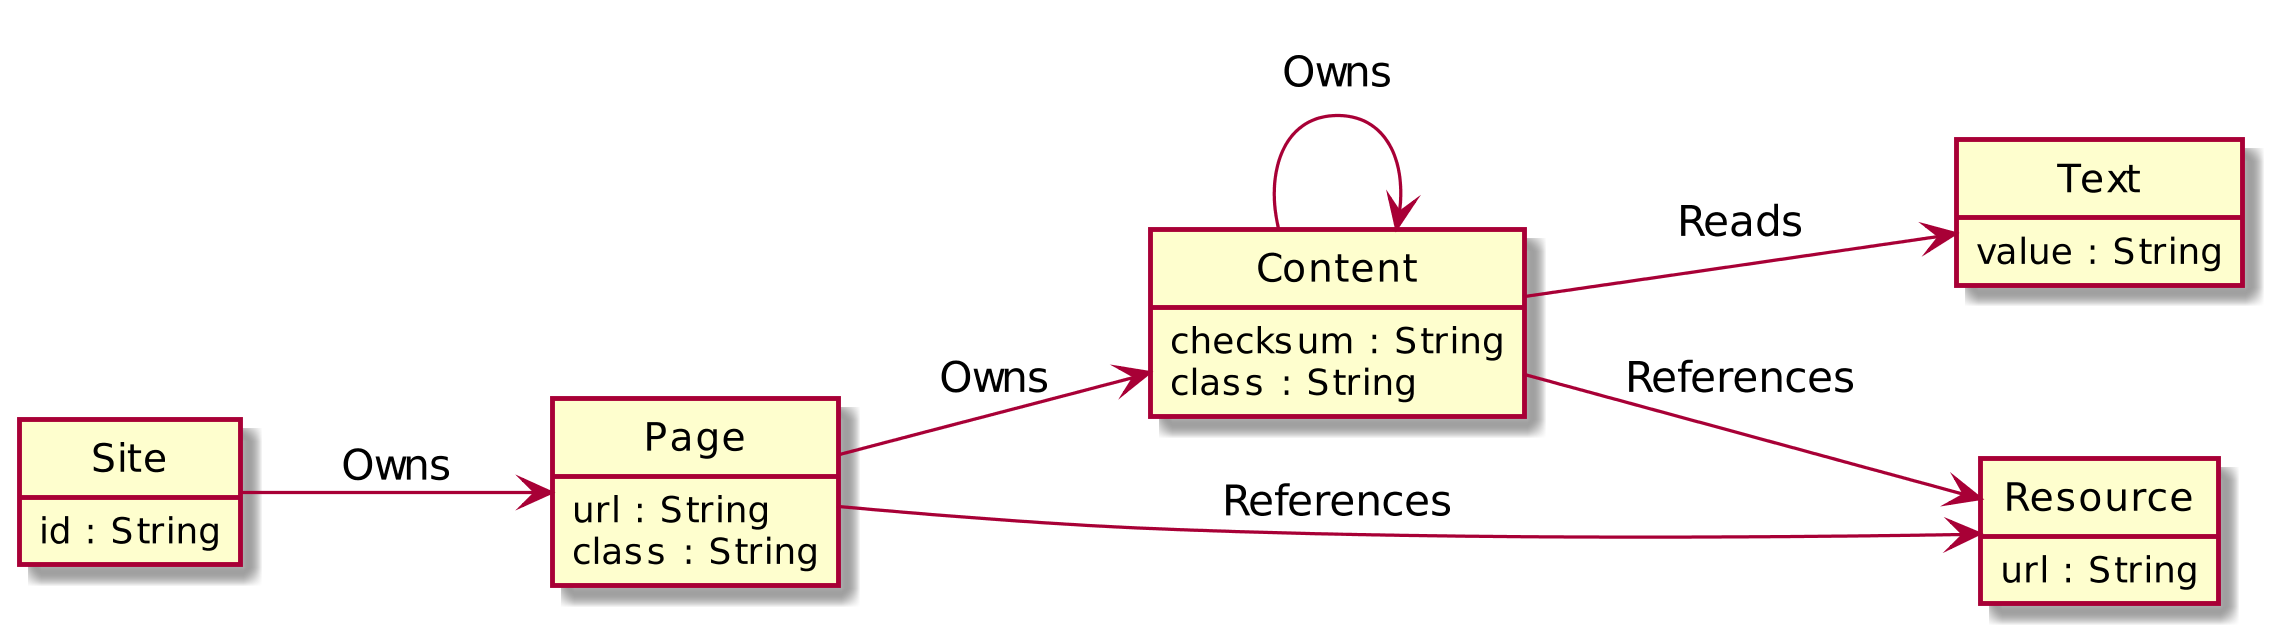
\includegraphics[width=\textwidth]{../resources/db-data-model/nodes.png}
        \caption{Übersicht der Nodes und ihrer Beziehungen}
        \label{image:dbDataModelOverview}
    \end{figure}

    Entitäten, die als Node umgesetzt werden, sind Seiten, Content Features,
    der Text eines Content Features, referenzierte {\resources} und Sites.
    Diese erhalten die entsprechenden Labels Page, Content, Text, Reference und Site.
    Eine Seite kann als {\resource} existieren, bevor sie selbst klassifiziert wird.
    In diesem Fall erhält der Knoten zum Zeitpunkt der Klassifizierung zusätzlich auch das Label Page.

    Ein Seitenknoten speichert die \gls{url} der Seite, die auch als eindeutiger Identifier innerhalb der Datenbank dient,
    und die Klasse der Seite.

    Der Knoten einer {\resource} enthält lediglich ihre \gls{url}, die wiederum als eindeutiger Schlüssel dient.
    Wie später deutlich wird, kann er für alle Referenzen, die diese {\resource} als Ziel haben, genutzt werden.

    Knoten mit dem Label "`Content"' enthalten eine Prüfsumme über sich selbst, die innerhalb der Datenbank als Schlüssel Verwendung findet.
    Im späteren Verlauf geht Kapitel \ref{section:solutionDetailsStorageAPIStoreClassification} darauf ein,
    wieso diese Eigenschaft des Weiteren benötigt wird.
    Für skalare Content Features existiert exakt ein Knoten.
    Für CollectionFeatures existiert ein Knoten pro Element der Liste.

    Der Text eines Content Featuers wird in einem separaten Knoten gespeichert,
    der neben dieser Information nichts speichert und deshalb auch eindeutig über den Text identifiziert wird.
    Zwischen diesen beiden Knoten existiert deshalb eine Beziehung, die das Label Reads besitzt.
    Jeder Content Knoten ist maximal mit einem Textknoten verbunden.
    Der Grund für die Auslagerung ist, dass es viele Features geben kann, die den gleichen textuellen Inhalt besitzen.
    Die Intention ist diese Eigenschaft im Graphen explizit zu machen,
    sodass sie leicht für komplexere Analysen genutzt werden kann.
    Ein Anwendungsfall ist z. B. Informationen aus einer Datenbank,
    die auf verschiedene Seiten ausgegeben werden.
    Ein Text Knoten hat in diesem Fall viele eingehende Beziehungen,
    sodass leicht herausgefunden werden kann, auf welchen Seiten er enthalten ist.
    Eine explizite Beziehung ist dabei semantisch ausdrucksstärker und effizienter,
    als ein einfacher String-Vergleich, der über mit allen Knoten gemacht wird.
    Durch die Beziehung hat man die Info direkt.
    String-Vergleich ist auch dann nicht mehr sinnvoll, wenn man alle Knoten haben möchte,
    die sich einen Text teilen.
    Dann müsste man sehr viele Vergleiche durchführen.
    Durch die Beziehung ist es einfach nur alle Text Nodes, die mehrere einkommende Kanten haben.

    Zu guter Letzt speichern Site Knoten die ID der Site, wodurch der Knoten eindeutig identifiziert wird.
    Jede Seite kann mit beliebig vielen Page Knoten verbunden sein.
    Diese Beziehungen haben das Label Owns.

    Sowohl Seiten als auch Content Features können Content Features enthalten.
    Eine Seite ist zu jedem Content Feature mit einer eigenen Beziehung verbunden,
    die ebenfalls das Label Owns besitzt.
    Das gleiche gilt für Contents und ihre eigenen Content Features.
    Eine genauere Darstellung dieser Beziehung bietet Abbildung \ref{image:dbDataModelContentRelationship}.

    \begin{figure}
        \centering
        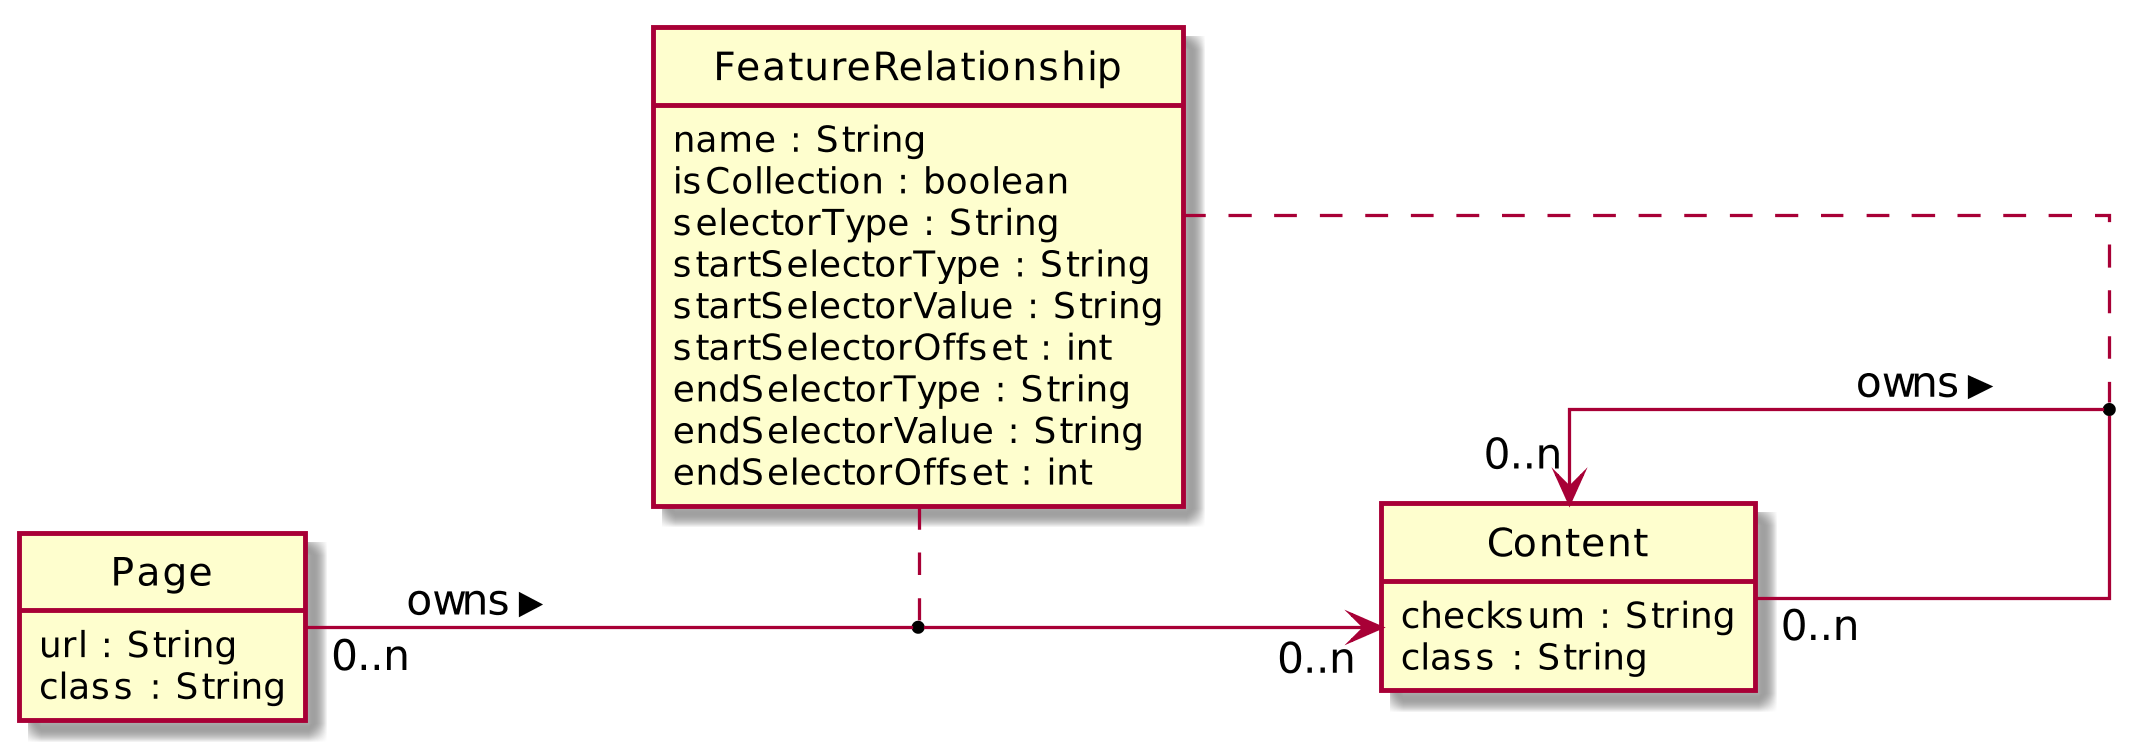
\includegraphics[width=\textwidth]{../resources/db-data-model/content-relationship.png}
        \caption{Content Features}
        \label{image:dbDataModelContentRelationship}
    \end{figure}

    Eine Beziehung zwischen Page und Content bzw. Content und Content
    wird hier als FeatureRelationship bezeichnet.
    Eine solche Beziehung besitzt eine Reihe von Eigenschaften.
    Sie speichert den Namen des Features (name),
    ob es sich um ein Element eines CollectionFeatures handelt (isCollection)
    und den eindeutigen Selektor des Nodes, der zum Feature gehört
    (start-, endSelectorType; start-, endSelectorValue; start- endSelectorOffset, ).
    Bei Collection Features existieren viele ausgehende Kanten für ein Feature.
    Jede dieser Beziehungen speichert den gleichen Namen und hat isCollection auf true gesetzt.
    Es ist sinnvoll diese Informationen nicht im Content Knoten, sondern in der Beziehung zu speichern,
    um den Knoten besser wiederverwendbar zu machen.
    Details werden in Kapitel \ref{section:solutionDetailsStorageAPIStoreClassification} erklärt.

    Referenzen werden in der Datenbank durch eine Kombination aus
    {\resource} Knoten und Beziehungen zu diesen Knoten dargestellt.
    Page und Content Knoten können demanch eine ausgehende Beziehung zu einem
    {\resource} Knoten haben, die mit References markiert ist.
    Abbildung \ref{image:dbDataModelResourceRelationship} stellt diese Beziehung in den Fokus.

    \begin{figure}
        \centering
        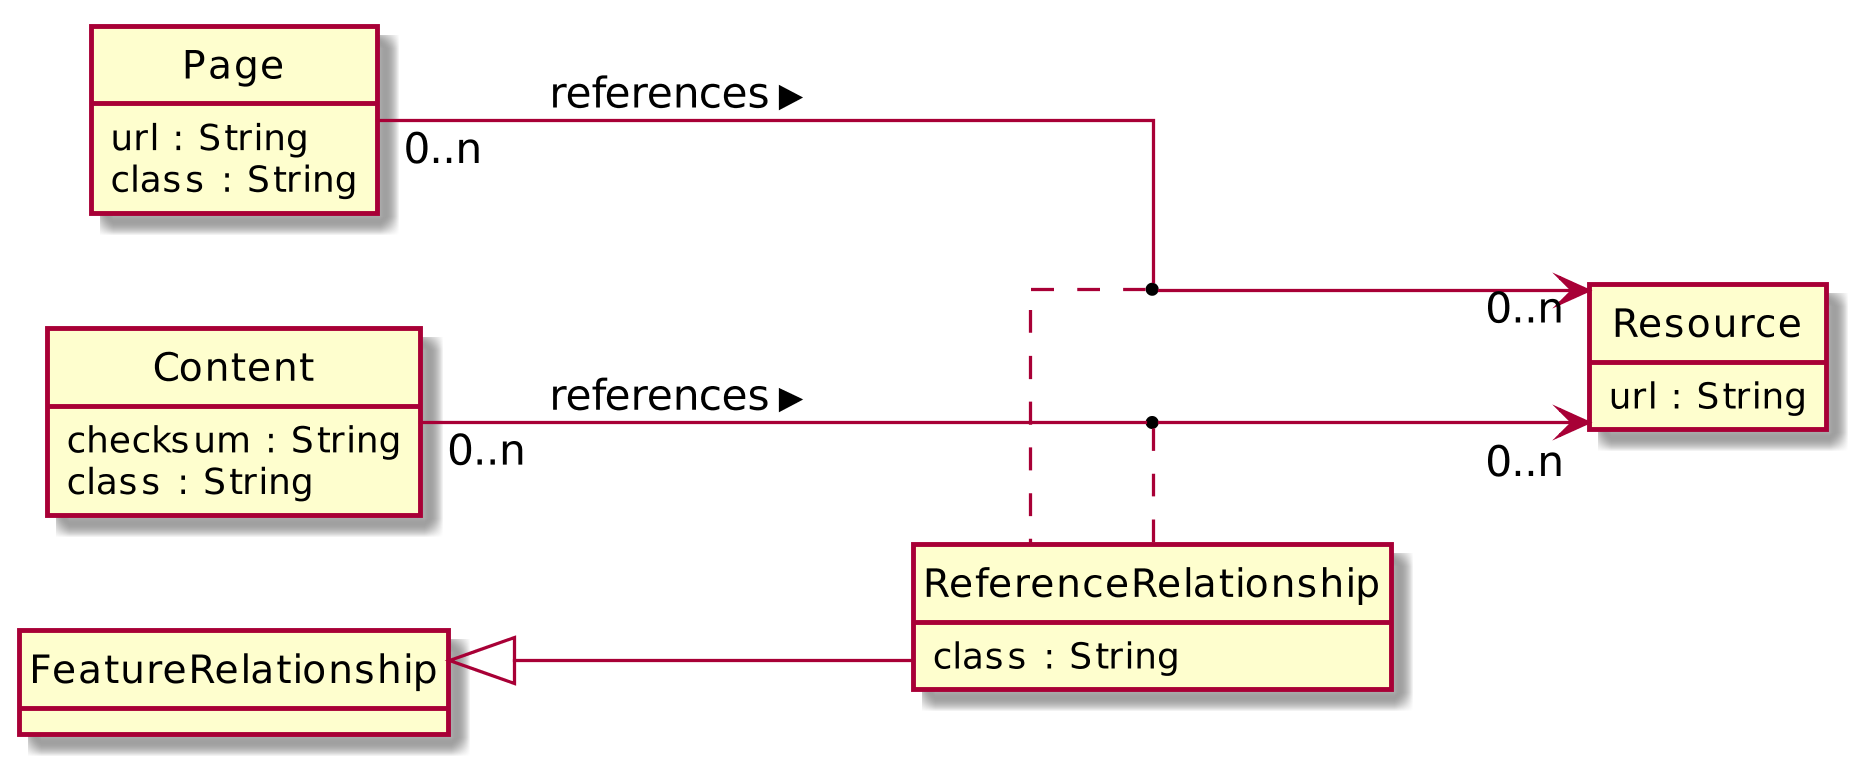
\includegraphics[width=\textwidth]{../resources/db-data-model/resource-relationship.png}
        \caption{Reference Features}
        \label{image:dbDataModelResourceRelationship}
    \end{figure}

    Wie zu sehen ist, handelt es sich bei einer ReferenceRelationship ebenfalls
    um eine FeatureRelationship, weshalb sie ebenfalls die oben beschriebenen Informationen speichert.
    Zusätzlich enthält sie aber auch die Klasse der Referenz.
    Diese kann nicht im {\resource} Knoten gespeichert werden,
    da der Knoten für viele Referenzen dienen kann und die Klasse nicht überall identisch sein muss.